\begin{figure*}[t]
\centering
\subfloat[Prompt Stress Tests\label{tab:prompt_stress_test_rolewise}]{\parbox[t][2.9cm][t]{0.24\textwidth}{\centering\vspace*{0.3cm}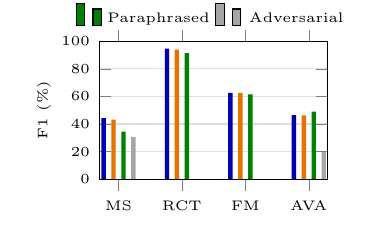
\begin{tikzpicture}\begin{axis}[ymajorgrids, grid style={gray!25}, tick label style={font=\tiny}, label style={font=\tiny}, title style={font=\tiny}, legend style={font=\tiny, draw=none, fill=none, at={(0.5,1.02)}, anchor=south}, legend columns=3, scale only axis, width=2.9cm, height=1.75cm, legend style={overlay}, ylabel shift=-3pt, ybar, bar width=1.6pt, symbolic x coords={MS,RCT,FM,AVA}, xtick={MS,RCT,FM,AVA}, ylabel={F1 (\%)}, ymin=0, ymax=100, legend columns=2]\addplot[fill=blue!70!black,draw=none] coordinates {(MS,44.35)(RCT,94.69)(FM,62.68)(AVA,46.51)};\addplot[fill=orange!90!black,draw=none] coordinates {(MS,43.11)(RCT,93.91)(FM,62.64)(AVA,46.29)};\addplot[fill=green!50!black,draw=none] coordinates {(MS,34.46)(RCT,91.44)(FM,61.61)(AVA,48.97)};\addplot[fill=gray!70,draw=none] coordinates {(MS,30.59)(AVA,19.71)};\legend{Original,Cue-masked,Paraphrased,Adversarial}\end{axis}\end{tikzpicture}}}\hfill
\subfloat[Macro-F1 vs.\ Threshold\label{fig:tau}]{\parbox[t][2.9cm][t]{0.24\textwidth}{\centering\vspace*{0.3cm}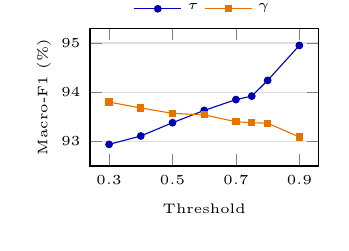
\begin{tikzpicture}\begin{axis}[ymajorgrids, grid style={gray!25}, tick label style={font=\tiny}, label style={font=\tiny}, title style={font=\tiny}, legend style={font=\tiny, draw=none, fill=none, at={(0.5,1.02)}, anchor=south}, legend columns=3, scale only axis, width=2.9cm, height=1.75cm, legend style={overlay}, ylabel shift=-3pt, xlabel={Threshold}, xtick={0.3,0.5,0.7,0.9}, legend columns=2, ylabel={Macro-F1 (\%)}, ymin=92.5, ymax=95.3]\addplot[mark=*,mark size=1.2pt,color=blue!70!black] coordinates {(0.3,92.94)(0.4,93.11)(0.5,93.38)(0.6,93.63)(0.7,93.85)(0.75,93.92)(0.8,94.24)(0.9,94.95)};\addplot[mark=square*,mark size=1.1pt,color=orange!90!black] coordinates {(0.3,93.80)(0.4,93.68)(0.5,93.57)(0.6,93.54)(0.7,93.40)(0.75,93.38)(0.8,93.37)(0.9,93.09)};\legend{$\tau$,$\gamma$}\end{axis}\end{tikzpicture}}}\hfill
\subfloat[Corpus Size vs.\ Threshold\label{fig:gamma}]{\parbox[t][2.9cm][t]{0.24\textwidth}{\centering\vspace*{0.3cm}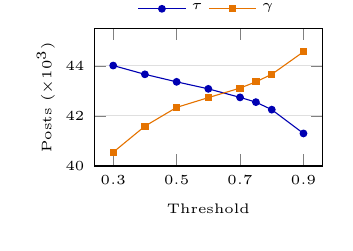
\begin{tikzpicture}\begin{axis}[ymajorgrids, grid style={gray!25}, tick label style={font=\tiny}, label style={font=\tiny}, title style={font=\tiny}, legend style={font=\tiny, draw=none, fill=none, at={(0.5,1.02)}, anchor=south}, legend columns=3, scale only axis, width=2.9cm, height=1.75cm, legend style={overlay}, ylabel shift=-3pt, xlabel={Threshold}, xtick={0.3,0.5,0.7,0.9}, legend columns=2, ylabel={Posts ($\times10^3$)}, ymin=40, ymax=45.5]\addplot[mark=*,mark size=1.2pt,color=blue!70!black] coordinates {(0.3,44.01)(0.4,43.66)(0.5,43.36)(0.6,43.08)(0.7,42.74)(0.75,42.55)(0.8,42.25)(0.9,41.30)};\addplot[mark=square*,mark size=1.1pt,color=orange!90!black] coordinates {(0.3,40.55)(0.4,41.59)(0.5,42.34)(0.6,42.73)(0.7,43.11)(0.75,43.36)(0.8,43.66)(0.9,44.56)};\legend{$\tau$,$\gamma$}\end{axis}\end{tikzpicture}}}\hfill
\subfloat[Parser Tolerance $\lambda$\label{fig:lambda}]{\parbox[t][2.9cm][t]{0.24\textwidth}{\centering\vspace*{0.3cm}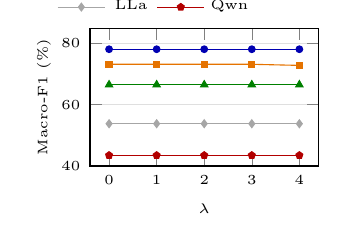
\begin{tikzpicture}\begin{axis}[ymajorgrids, grid style={gray!25}, tick label style={font=\tiny}, label style={font=\tiny}, title style={font=\tiny}, legend style={font=\tiny, draw=none, fill=none, at={(0.5,1.02)}, anchor=south}, legend columns=3, scale only axis, width=2.9cm, height=1.75cm, legend style={overlay}, ylabel shift=-3pt, xlabel={$\lambda$}, xtick={0,1,2,3,4}, ylabel={Macro-F1 (\%)}, ymin=40, ymax=85]\addplot[mark=*,mark size=1.2pt,color=blue!70!black] coordinates {(0,78.14)(1,78.14)(2,78.14)(3,78.14)(4,78.14)};\addplot[mark=square*,mark size=1.1pt,color=orange!90!black] coordinates {(0,73.22)(1,73.22)(2,73.22)(3,73.22)(4,72.86)};\addplot[mark=triangle*,mark size=1.5pt,color=green!50!black] coordinates {(0,66.53)(1,66.53)(2,66.53)(3,66.53)(4,66.53)};\addplot[mark=diamond*,mark size=1.4pt,color=gray!70] coordinates {(0,53.81)(1,53.81)(2,53.81)(3,53.81)(4,53.81)};\addplot[mark=pentagon*,mark size=1.3pt,color=red!70!black] coordinates {(0,43.50)(1,43.50)(2,43.50)(3,43.50)(4,43.50)};\legend{GPT,Mis,Gem,LLa,Qwn}\end{axis}\end{tikzpicture}}}
\caption{Robustness and sensitivity. (a)~Per-role F1 averaged over the five zero-shot classifiers on original, cue-masked, paraphrased, and adversarially rewritten evaluation posts; roles with fewer than 30 valid rewrites per classifier are omitted. (b, c)~RoBERTa Macro-F1 and size of the re-selected corpus as the topical relevance threshold $\tau$ and the role-exclusion threshold $\gamma$ vary (defaults $\tau{=}0.50$, $\gamma{=}0.75$). (d)~Zero-shot Macro-F1 as the parser tolerance $\lambda$ varies ($\lambda{=}2$ is used throughout). The lexicon threshold $\delta$ is not shown: across $\delta\in[0,0.1]$ it changes the corpus by at most 108 posts and Macro-F1 by at most 0.1 points.}
\label{fig:robustness}
\label{fig:delta}
\vspace{-0.3cm}
\end{figure*}